% The short-comings of other solutions are somewhat a continuation of the problem description

% * things from the knowledge-base: redux, flux, angular, meteor, linked-data
%    * instead of in problem-description (more abstract there)
\chapter{State of the Art}

\section{Frameworks and Architecture}

\subsection{Model-View-Controller}

You probably already are familiar with the classical model-view-controller architecture, but for the sake of completeness a short overview will be given here. The pattern mainly consists of three types of building blocks (as can also be seen in figure \ref{fig:mvc}):

\begin{description}
  \item[controllers] contain the lion's share of the business logic. User input gets handled by them and they get to query the model. Depending on these two information sources they decide what messages to send to the the model, i.e. the controller telling the model to change. Usually there's one controller per view and vice-versa.
  \item[models] hold the application's state and make sure it's consistent. If something in the data changes, it notifies views and controllers depending on it. These notifications can be parametrized, telling the dependants what changed.
  \item[views] are what the outside world/user's get to see. When the model changes, the view get's notified and -- depending on the data passed along and what it reads from the model --  updates accordingly.
  Especially in html-applications, views (and thereby controllers) tend to be nested (e.g. the entire screen, a column, a widget in it, a button in the widget)
\end{description}

Note that there's a wide range of different instances/interpretations of the architectural patterns can organise models/views/controllers differently. Further down, in section \ref{ref:angular-mvc} you can find one of these (angular's MVC) described in more detail.

\begin{figure*}
\centering
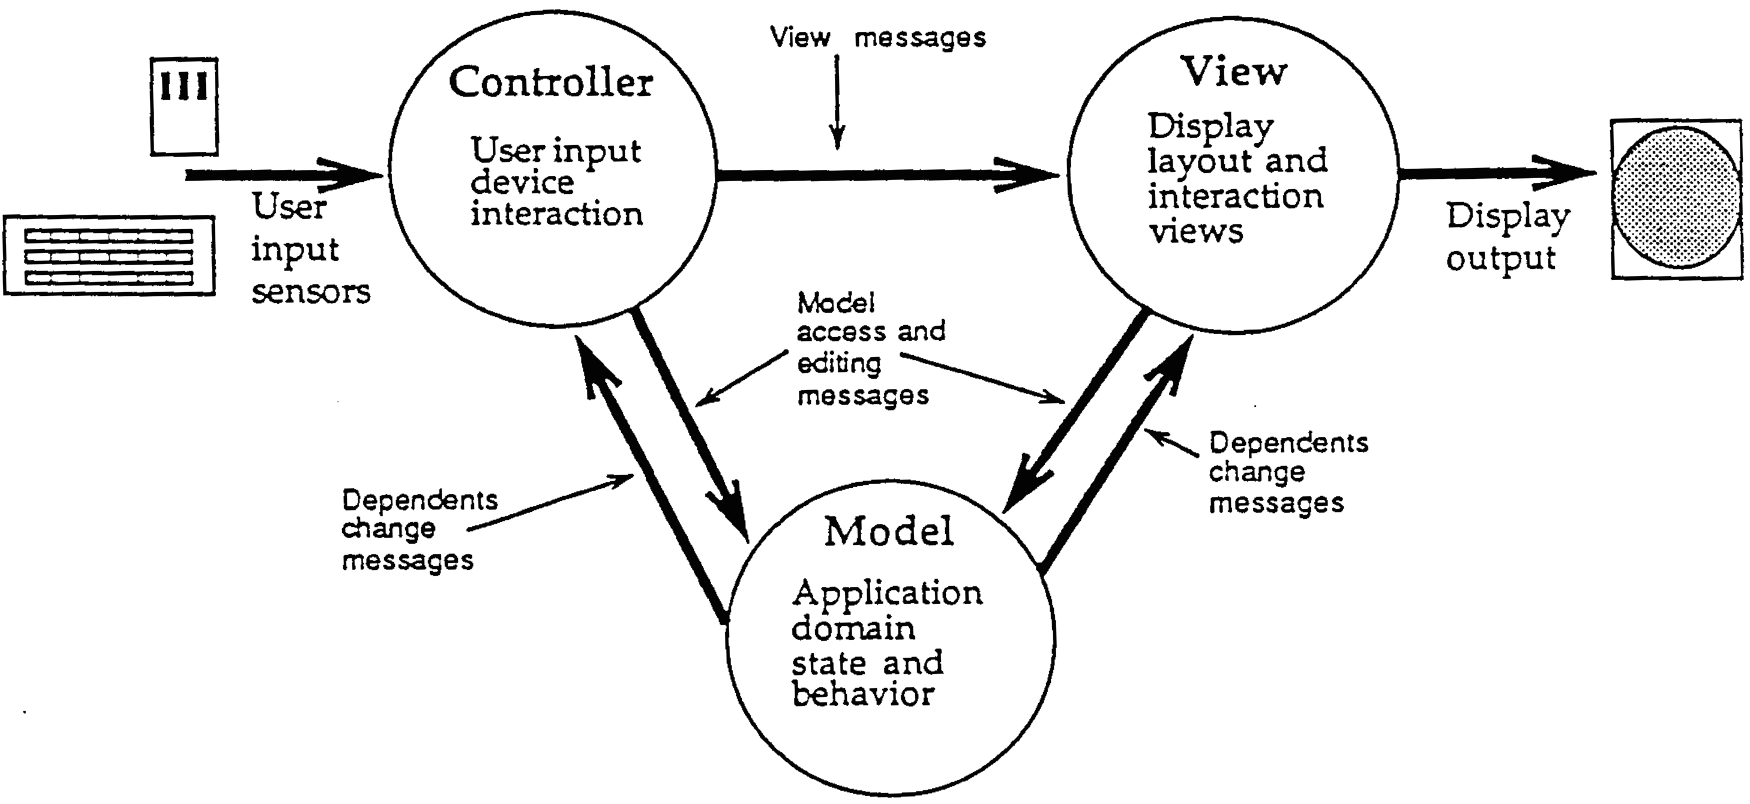
\includegraphics[width=1.0\textwidth]{figures/mvc.png}
\caption[MVC-architecture]{MVC-architecture (Krasner and Pope, 1988)}
\label{fig:mvc}
\end{figure*}
% TODO krasner and pope 1988: http://heaveneverywhere.com/stp/PostScript/mvc.pdf

\subsection{Model-View-ViewModel}

This architectural pattern, also known as ``Model-View-Binder'', is similar to MVC but puts more emphasis on the seperation between back-end and front-end. It's parts are as follows (and can be seen in fig. \ref{fig:mvvm}):

\begin{description}
  \item[The model] is the back-end business-logic and state. It can be on a different machine entirely.
  \item[The view-model] contains the front-end logic and state. It is a thin binding layer, that processes inputs and that manages and provides the data required by the view.
  \item[The view] is a stateless rendering of the data retrieved from the view-model; in the case of some frameworks, this happens via declarative statements in the view's templates, that automatically get updated when the data in the view-model changes. User-input events raised in the view get forwarded to the view-model.
\end{description}

\begin{figure*}
\centering
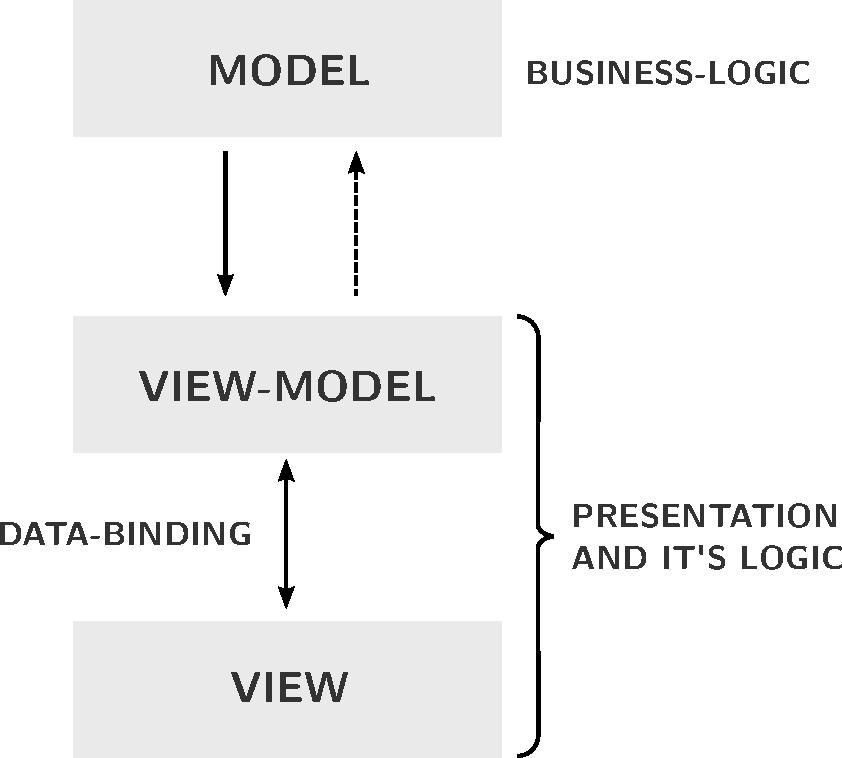
\includegraphics[height=8cm]{figures/mvvm.pdf}
\caption[MVC-architecture]{ MVVM-architecture (diagram \href{https://en.wikipedia.org/wiki/File:MVVMPattern.png}{adapted from wikimedia}\footnotemark{})}
\label{fig:mvvm}}
\end{figure*}
\footnotetext{\url{https://en.wikipedia.org/wiki/File:MVVMPattern.png}}

\subsection{Angular 1.x MVC}\label{ref:angular-mvc}

\begin{comment}
  * arguably more mvvm than mvc
  * rather steep learning curve. especially to use it well. there's many pitfalls for people just starting out with it to produce a code-base that's hard to maintain later on. (personal experience with smartengine-code and own code)
  * bi-directional binding
  * auto-injection into scope via things like ng-model
  * scoping / hierarchy of controllers
  * modules and dependency-injection
    * need to include each and every javascript file (in the right order?). everything is loaded with quite a few http-requests. can be bundled though
      * make sure to use strict mode to allow bundling
    * no tree-shaking
    * redundant to es6-module system
  * services
    * keep global state
    * wrap access utilities to server-APIs
    * access to utility functions that can be injected (instead of being attached to the window)
  * controllers
    * both controllers and partly models (is angular actually mvvm?)
    * can be reused with different template, but that rarely happens and tends to lead to hard-to-track-down bugs.
    * mostly used at view level. below that directives provide more atomic bundling of template and code.
  * templates
  * filters
    * { probably not necessary to explain }
  * directives
    * bundle controller and template in one file
    * register custom html-tag (unless used in attribute, like ng-show/-class/-..., or class mode)
  * routing
    * html-fragments
    * ui-router (?) (are we using or have we used it?)
\end{comment}

\subsection{Meteor}

% dunno if necessary?

\subsection{React}

\begin{comment}
  * atomic components
  * vdom allows not needing to deal with dom-state just with defining one mapping from app-state to desired html. react takes care of calculating a minimal set of updates (by diff'ing the current vdom against the vdom that produced the previous dom-state (?))
\end{comment}

\subsection{Flux}

\begin{comment}
  * quite a learning-curve
  * actions
  * dispatcher
    * there are many different implementations of these (the one by fb, the one by yahoo,...)
  * stores
    * waitFor
    * dependencies between these can be hard to understand
    * lot of overhead
    * side-effect free? if so, do as much as business logic as possible here.
  * views
    * most dispatchers / setups are geared to be used with redux
\end{comment}


\subsection{Redux}\label{ref:redux}

\begin{comment}
  * http://redux.js.org/
  * can be super-simple (give trivial example)
  * easy to learn (it's only one event-bus/dispatcher, one reduction-function)
  * ideally used with immutable data for model (to avoid bugs due to pass-by-reference and later modification)
  * doesn't deal with side-effects by default (see ACs and actors later)
  * (action-creators (for pre-processing))
  * actions
  * dispatcher
  * reduction function
    * synchronous (can't do asynch side-effects here)
    * (supposed to be) side-effect free. do as much as business logic as possible here.
  * components
\end{comment}

\subsection{Ng-Redux}\label{ref:ng-redux}

\begin{comment}
  * https://github.com/wbuchwalter/ng-redux
  * angular 1.X for rendering instead of flux
  * good for migrating
  * duplicate imports if using es6 (though not ng-redux inherent)
  * explain binding into routing, setup of watches, importance of one way bindings
\end{comment}


\subsection{Elm}

\begin{comment}
  * previous (at time of designing)
  * current
\end{comment}

\subsection{CycleJS MVI}

\begin{comment}
* driver's are similiar to actors?
\end{comment}

% move this to methodology chapter?

% http://redux.js.org/
% https://github.com/angular-redux/ng-redux
